\documentclass[12]{beamer}

\author{Pritvi Jheengut @zcoldplayer}
\title{My experience as a Level 8 Google Maps Local Guide}

\usepackage[T1]{fontenc}
\usepackage[utf8]{inputenc}
\usepackage[size=a4, orientation=landscape, scale=3.5]{beamerposter}

\usepackage{lmodern}
\usepackage{fontenc}[T1]
\usepackage{inputenc}[utf8]
\usepackage{hyperref}[pdfpagelabels=true,bookmarks=true,unicode=true]

\usepackage{pgf}
\usepackage{verbatim}

\usepackage{listings}
\usepackage{xy}[all]

% Eliminate errors such as
% LaTeX Font Warning: Font shape `T1/cmss/m/n' in size <4> not available
% LaTeX Font Warning: Size substitutions with differences up to 1.0pt 

\usepackage{graphicx}
\usepackage{booktabs}

\mode<presentation>{
  
  \useoutertheme{infolines}
  \usecolortheme{whale}
  
%   \definecolor{ncurses}{HTML}{BBFFFF}
%   \definecolor{darkblue}{HTML}{33AA88}
  \definecolor{light}{HTML}{0088FF}
  \definecolor{confblue}{HTML}{55AAFF}
  
  \setbeamercolor{Title bar}{fg=black!90}
  \setbeamercolor{frametitle}{parent=black,bg=confblue,fg=black!70}
  \setbeamercolor{titlelike}{parent=light,bg=confblue!40,fg=black!85}
  \setbeamercolor{block title}{bg=confblue,fg=yellow}
  
  \setbeamercovered{transparent,dynamic}
  
  \setbeamertemplate{blocks}[rounded][shadow=true]
  \setbeamertemplate{background canvas}[vertical shading]
  [top=red!45,middle=light!35,bottom=confblue!50]
  
  % \mode<handout>{\beamertemplatesolidbackgroundcolor{black!50}}
  
}

\subtitle{An insight of Google Maps and associated key technologies for 
Local Guides while setting up ratings, reviews, multimedia, missing 
places, 
answers, questions within Google Maps as well as the benefits of 
becoming a Google Local Guide Contributor.} 

% \date{ }

\begin{document}
  
  \date[]{}
  
  \maketitle
  
  \section{CopyLeft License}
  
  \frame{
    \frametitle{Copyleft License Attribution}
    
    Made with love using beamer, LaTeX and git.\\
    You can view at \href{https://gitlab.com/Presentation-PritviJheengut/
    local-guide-google-maps-contributor/}{
    local-guide-google-maps-contributor}
    
    \begin{alertblock}{This work is licensed under the LaTeX Project
        Public License.}
      To view a copy of this license, visit \\
      \url{https://www.latex-project.org/lppl.txt} 
    \end{alertblock}
    
    \begin{alertblock}{This work is licensed under the Creative
        Commons Attribution 4.0 International License.}
      To view a copy of this license, visit \\
      \url{http://creativecommons.org/licenses/by/4.0/} or \\
      
      send a letter to \\
      Creative Commons, \\
      PO Box 1866, \\
      Mountain View, \\
      CA 94042, \\
      USA. \\
    \end{alertblock}
  }

  \section{Greetings}
  
  \frame{
    \frametitle{Who Am I}
    
    \large
    
    \href{http://slackware.com/}{Geek@Slackware}
    
    \href{https://twitter.com/zcoldplayer}{twitter @zcoldplayer}
    
    \href{https://xmail.net/z.coldplayer}{zcoldplayer xmail Website}
    
    \href{http://metservice.intnet.mu/}{Work
    : SMTT@Meteorological.Services.mu}
    
    Active in many User group LUGM, MMC, MSCC, FECM, GDG\_MU \\
    and several other hackathons
    
    Passionate about how and why things work.
    
    Fervour Advocate of Free Libre and Open Source Software.
    
    \href{https://maps.google.com/localguides/home}{Pritvi 
    Jheengut - Level 8 Google Maps Local Guide}
    
  }
  
  \frame{
    \frametitle{Who are you}
    
    \large
    
    \begin{block}{Would you mind tell me who you are?}
      \begin{enumerate}
        \item @twitter\_handle
        \item where you work
        \item email you want to share
        \item Hobbies
        \item purpose and expectations of this session
      \end{enumerate}      
    \end{block}
    
  }
  
  \section{Community Groups in Mauritius}
  
  \frame{
    \frametitle{Community Groups in Mauritius}
    
    \begin{block}{Healthy growth of Community Groups in Mauritius}
      This turn of the century has seen an uprising of Community groups in
      Mauritius in the field of the Digital World. The diversity has 
      helped the exchange and sharing of innovative ideas, experience, 
      bleeding edge technology, upcoming events, conferences in the 
      Digital Island of the Republic of Mauritius.
    \end{block}
    
    \large
    
    This is a list of some of the active communities in Digital Mauritius.
    \begin{itemize}
      \item Linux User Group Meta, LUGM
      \item Mauritius Software Craftmanship Community, MSCC
      \item Mauritius Makers Community, MMC
      \item Front-End Coders Mauritius, FECM
      \item PHP User Group of Mauritius, phpMauritiusUG
      \item Symfonymu
      \item Google Developers Group Mauritius, GDG\_M
      \item Digital Marketing Mauritius
    \end{itemize}
    
  }
  
  \section{Introduction to Google Local Guides and Google Maps}
    
  \frame{
    \frametitle{About Google Local Guides}
    
    \large
    
    \begin{block}{Characteristics of a Local Guide}
    A person eager to share tips, make discoveries and share news and 
    other content with the community using
    
    \begin{itemize}
      \item knowledge
      \item photos
      \item reviews
      \item video
      \item questions
      \item multimedia
    \end{itemize}

    in order to better understand places is often a 
    \href{https://www.localguidesconnect.com/}{Local Guide.}
          
    More specifically, a Google Local Guide uses \href{maps.google.com}{
    Google Maps} for the above mentioned actions regularly.
    \end{block}

    }
    
  \frame{
    \frametitle{About Google Maps}
    
    \large
    
    \begin{block}{Google Maps is a GIS}
    Google Maps is a raster based Geographic Information System, ie GIS,
    available either as a Web App or as a Mobile App designed to present
    spatial or geographic data only.
    \end{block}
    
    \begin{block}{What is Google Maps after all?}
    Google Maps helps Local Guides to find geographic information based on
    what they are searching for and also where they are looking forward to
    go to with relevance to places they are interested in. 
    
    By the way, people other than Local Guides can use Google Maps too.
    \end{block}
    
    \begin{block}{Google Maps Local Guide Meetups}
    Google Maps provides Local Guides the ability to host or join
    \href{https://maps.google.com/localguides/meetup}{meetups}.
    \end{block}

    }
  
  \section{About Local Guides Connect}
  
  \frame{
    \frametitle{Local Guides Connect}
    
    \large
    
    \begin{block}{Regarding Local Guides Connect}
    When Google Maps is not enough for Local Guides.
    
    Sometimes Local Guides need more space to contribute to more than 
    just about places such as
    
    \begin{itemize}
      \item to talk about Google Maps, 
      \item write blogs about their experience
      \item add content that don't fit on a particular given location
      \item Tutorials, Manuals, How-Tos
      \item Stories
    \end{itemize}
    
    \end{block}
    
    }
    
  \frame{
    \frametitle{Local Guides Connect}
    
    \large
    
    \begin{block}{Local Guides Connect in depth}
    \href{www.localguidesconnect.com}{Local Guides Connect} provides more
    detailed post or blogpost such as
    
    \begin{itemize}
      \item Photography
      \item Travel
      \item Food and Drink
      \item Local Stories
      \item Meet-ups
      \item How-tos
      \item Announcements
      \item Help Desk
      \item Idea Exchange
    \end{itemize}
    
    \href{www.localguidesconnect.com}{This Webite localguidesconnect} is 
    the place to go to fulfil these needs.
    
    \end{block}
    
    }
    
    \section{Using and Contributing to Google Maps}
    
  \frame{
    \frametitle{Contributing on Google Maps}
    
    \begin{block}{Steps to Contributing to Google Maps}
    Contributing to Google Maps is easy and quite intuitive. Imparting
    knowledge, tips, multimedia content, new places, satisfaction of 
    visiting a particular place influence how other people.
    
    Here are the current ways of Contributing 

    \begin{itemize}
    \item Rate and write a Review, better if the Review in question is 
    more than 200 words
    \item Add Photos not just flat images but 360, panoramic too are 
    welcomed 
    \item Add Videos but there is a time limit of 30 seconds
    \item Answer questions about the particular place, tags are then 
    associated for quick look up by the Google search engine and also
    helpful for people with accessibility issues
    \item Add a place and edit places to correct mistakes or updating
    new information
    \item Check and verify facts about a recently added place before it is
    published on Google Maps, this is one of the reasons it takes hours 
    before a new place is available for Review
    \end{itemize}

     \href{
https://support.google.com/local-guides/answer/2519605?hl=en&ref_topic=6224
587}{Great tips for Local Guides}
    
    \end{block}

    }
    
  \frame{
    \frametitle{Benefits of Contributing}
    
    \begin{block}{Collect Points by Contributing to Google Maps}

    \begin{table}{Guide to acquire points }
    
    \centering
    \caption{Local Guides contribution points}
    
    \begin{tabular}{|l|r|}
    
    \toprule
    
    Maps contribution & Points earned \\
    
    \midrule
    
    Review & 10 points per review \\
    Review with more than 200 characters & 10 bonus points per review \\
    Rating & 1 point per rating \\
    Photo & 5 points per photo \\
    Video & 7 points per video \\
    Answer & 1 point per answer \\
    Respond to Questions and Answers & 3 points per response \\
    Edit & 5 points per edit \\
    Place added & 15 points per place added \\
    Road added & 15 points per road added \\
    Fact checked & 1 point per fact checked \\
    
    \bottomrule
    
    \end{tabular}
    
    \end{table}
    
    \href{https://maps.google.com/localguides/howto}{Local Guides Level
    badging}
    
     \href{
https://www.blog.google/products/maps/seven-kinds-local-guides-you-might-sp
ot-google-maps/}{Nice blog about types of local guides}
    
    \end{block}
    
    }
    
    \section{Badge Levels}
    
  \frame{
    \frametitle{Photographer}
    
    \begin{center}
    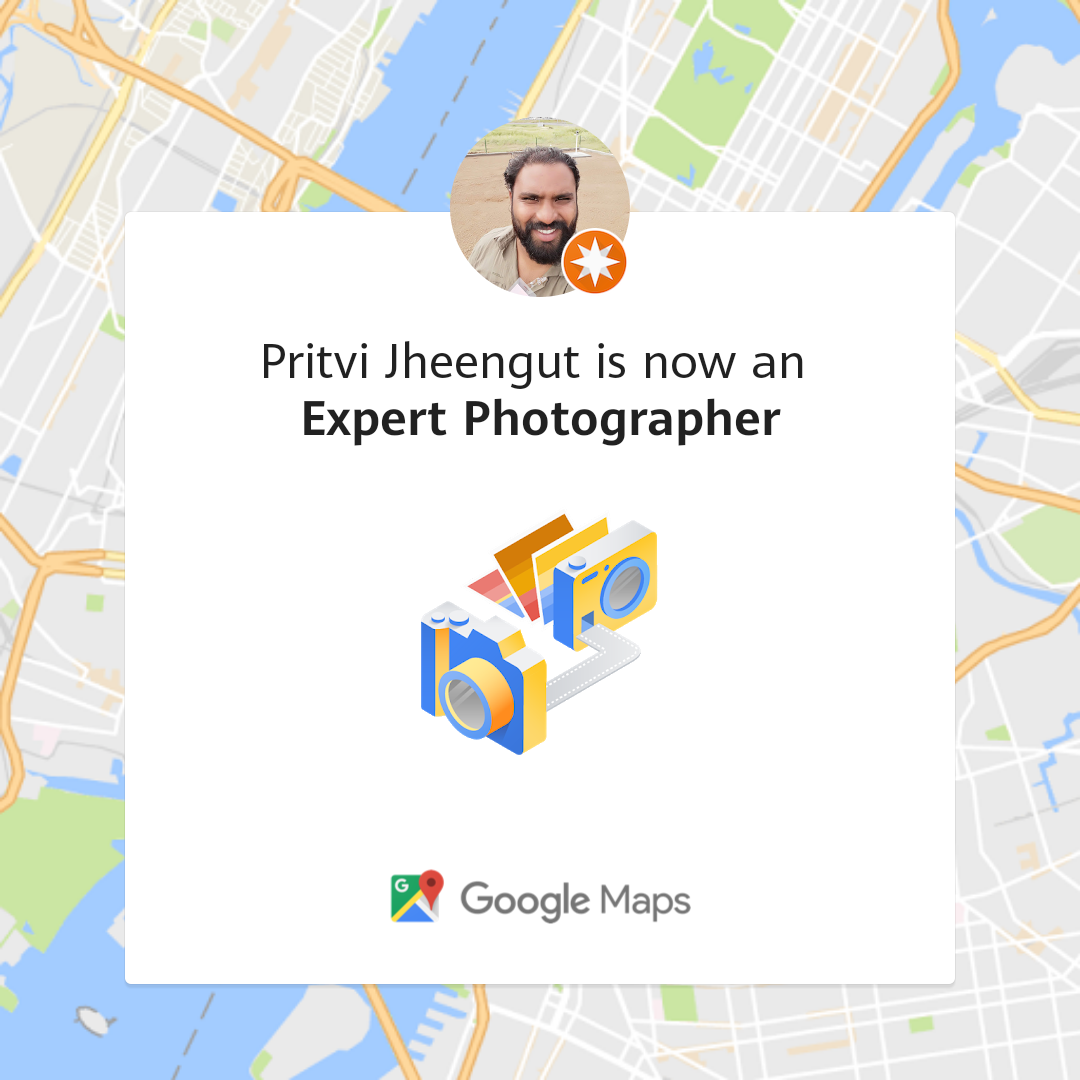
\includegraphics[height=.59\linewidth]{PNG/ExpertPhotographer.png}
    \end{center}
    
    }
    
  \frame{
    \frametitle{Photographer}
    
    \begin{table}{Guide to badge level for a Photographer}
    
    \centering
    \caption{Local Guides unlock points}
    
    \begin{tabular}{|l|r|}
    
    \toprule
    
    Photographer Level & Achiements acquired \\
    
    \midrule
    
    Novice & add photo of 3 places \\
    
    \midrule
    
    Expert & add 100 photos \\
    & add photos of 25 places \\
    & get 100000 photo views \\
    
    \midrule
    
    Master & add 1000 photos \\
    & add photos of 100 places \\
    & get 1M photo views \\
    
    \bottomrule
    
    \end{tabular}
    
    \end{table}
    
    }
    
  \frame{
    \frametitle{Reviewer}
    
    \begin{center}
    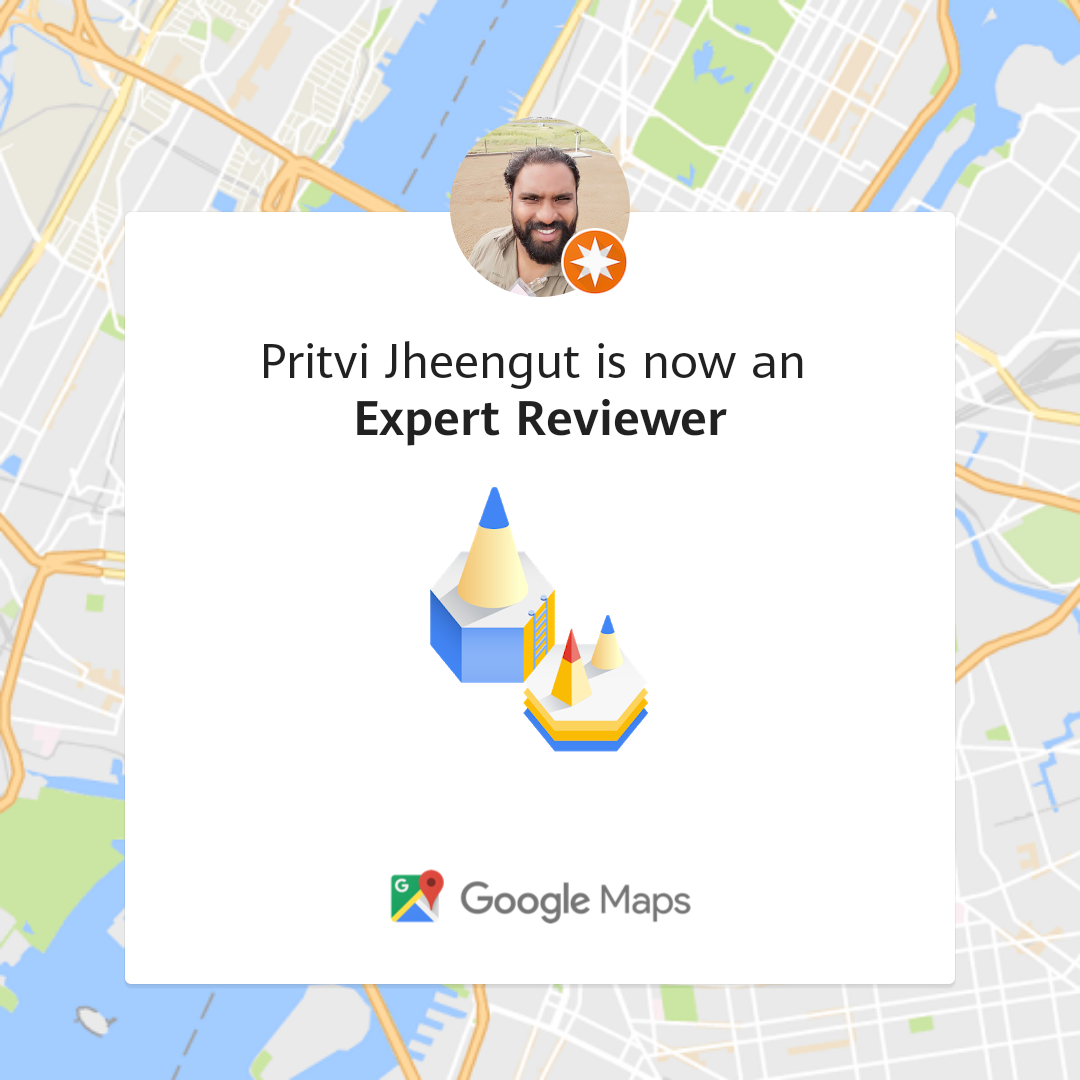
\includegraphics[height=.59\linewidth]{PNG/ExpertReviewer.png}
    \end{center}

    }
    
  \frame{
    \frametitle{Reviewer}
    
    \begin{table}{Guide to badge level for a Reviewer}
    
    \centering
    \caption{Local Guides unlock points}
    
    \begin{tabular}{|l|r|}
    
    \toprule
    
    Reviewer Level & Achiements acquired \\
    
    \midrule
    
    Novice & review 3 places \\
    
    \midrule
    
    Expert & review 3 places\\
    & write 5 reviews with over 200 characters \\
    & get 5 likes on your reviews \\
    
    \midrule
    
    Master & review 100 places\\
    & write 50 reviews with over 200 characters \\
    & get 50 likes on your reviews\\
    
    \bottomrule
    
    \end{tabular}
    
    \end{table}
        
    }
    
  \frame{
    \frametitle{Fact Finder}
    
    \begin{center}
    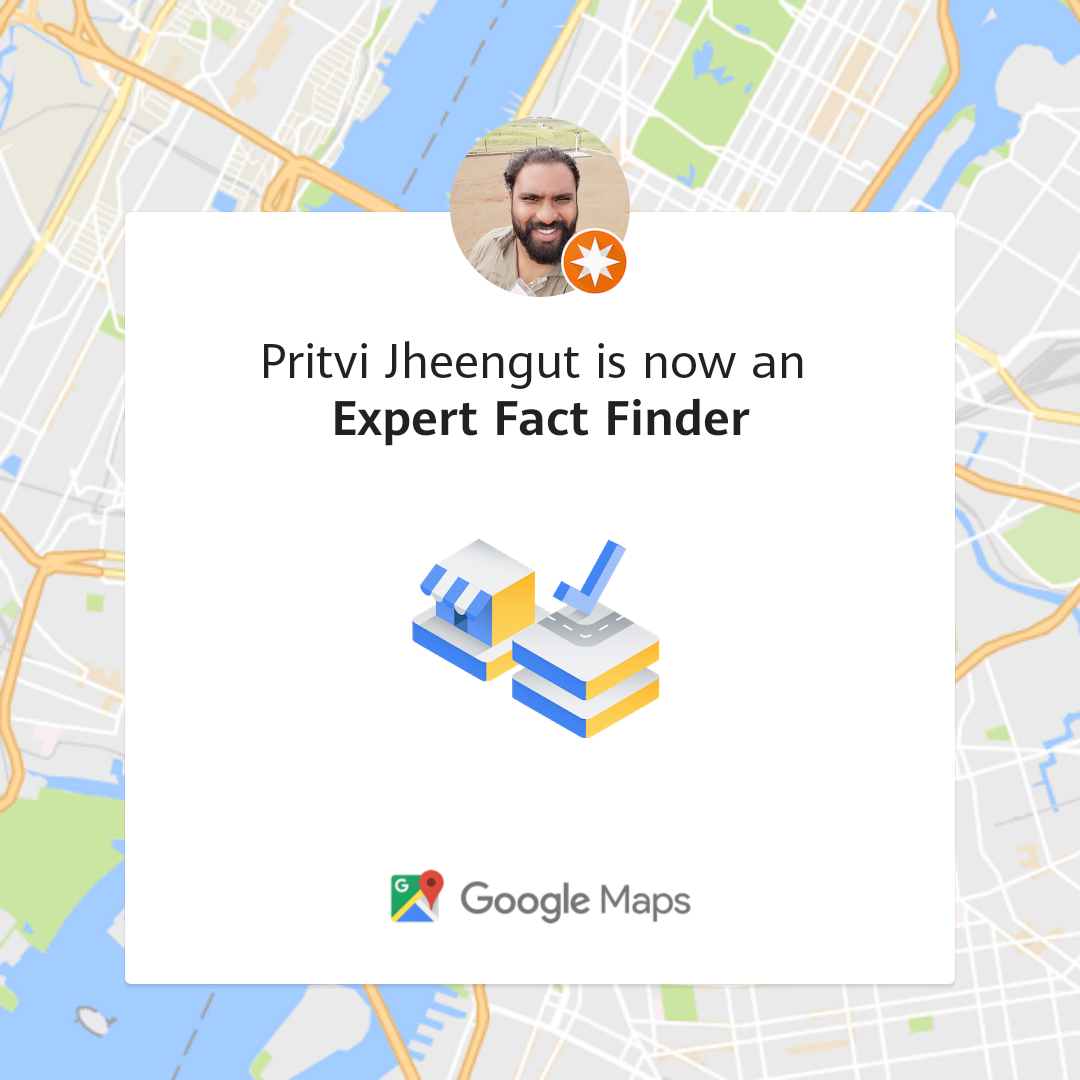
\includegraphics[height=.59\linewidth]{PNG/ExpertFactFinder.png}
    \end{center}

    }
    
  \frame{
    \frametitle{Fact Finder}
    
    \begin{table}{Guide to badge level for a Fact Finder}
    
    \centering
    \caption{Local Guides unlock points}
    
    \begin{tabular}{|l|r|}
    
    \toprule
    
    Fact Finder Level & Achiements acquired \\
    
    \midrule
    
    Novice & suggest 3 approved edits \\
    & verify 3 edits \\
    & answer 25 questions \\
    
    \midrule
    
    Expert & suggest 25 approved edits \\
    & verify 25 edits \\
    & answer 250 questions  \\
    
    \midrule
    
    Master & suggest 100 approved edits \\
    & verify 100 edits \\
    & answer 1000 questions  \\
    
    \bottomrule
    
    \end{tabular}
    
    \end{table}
        
    }
    
  \frame{
    \frametitle{Trailblazer}
    
    \begin{center}
    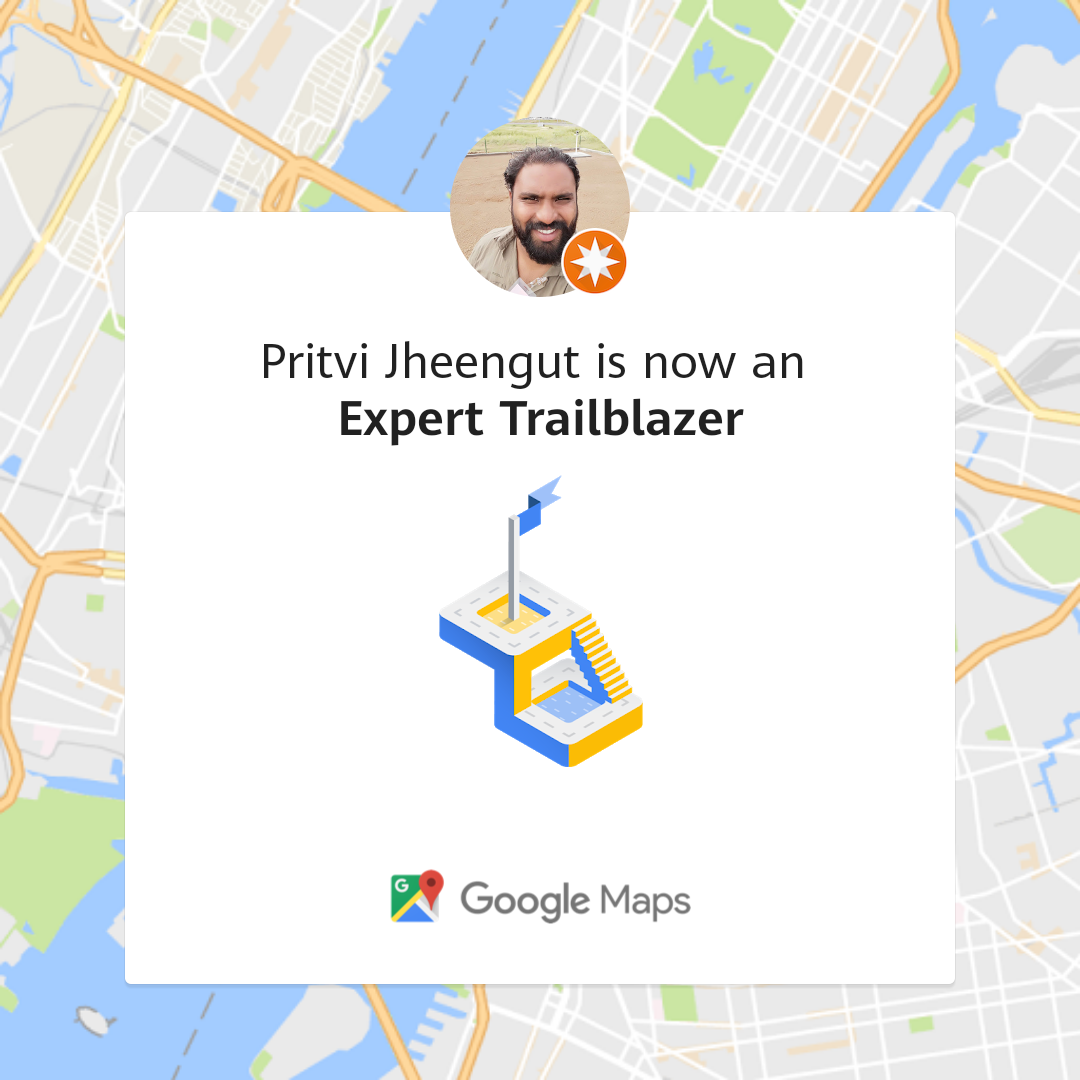
\includegraphics[height=.59\linewidth]{PNG/ExpertTrailblazer.png}
    \end{center}
    
    }
    
  \frame{
    \frametitle{Trailblazer}
    
    \begin{table}{Guide to badge level for a Fact Finder}
    
    \centering
    \caption{Local Guides unlock points}
    
    \begin{tabular}{|l|r|}
    
    \toprule
    
    Trailblazer Level & Achiements acquired \\
    
    \midrule
    
    Novice & add first photo of 1 place \\
    & write first review  of 1 place \\
    & add 1 approved place \\    
    
    \midrule
    
    Expert & add first photo of 10 places \\
    & write first review  of 10 places \\
    & add 10 approved places \\
    
    \midrule
    
    Master &  add first photo of 50 places \\
    & write first review  of 50 places \\
    & add 5- approved places \\
    
    \bottomrule
    
    \end{tabular}
    
    \end{table}
        
    }
    
  \frame{
    \frametitle{NoviceDirector}
    
    \begin{center}
    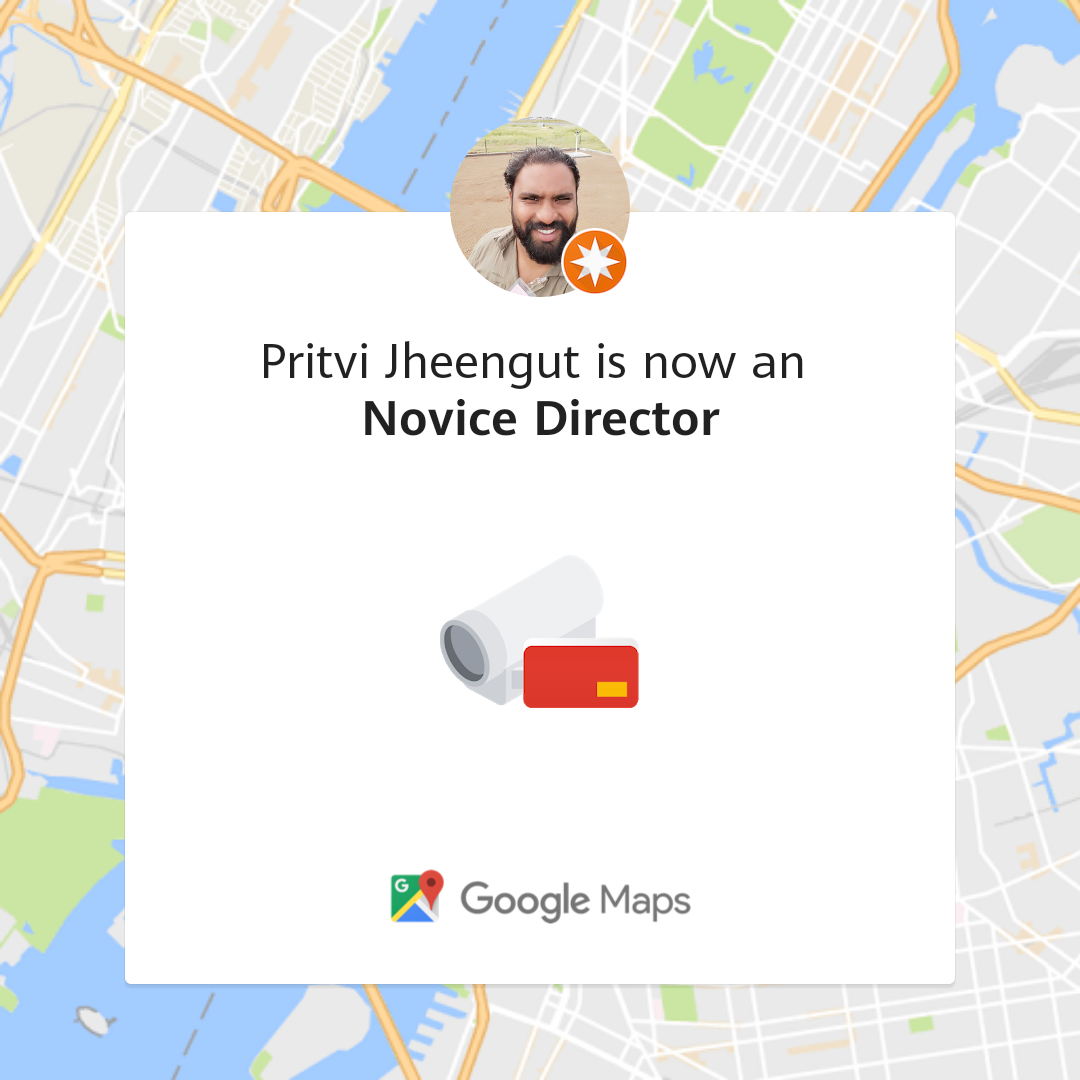
\includegraphics[height=.59\linewidth]{PNG/NoviceDirector.png}
    \end{center}
    
    }
    
  \frame{
    \frametitle{Novice Director}
    
    \begin{table}{Guide to badge level for a Novice Director}
    
    \centering
    \caption{Local Guides contribution points}
    
    \begin{tabular}{|l|r|}
    
    \toprule
    
    NoviceDirector Level & Achiements acquired \\
    
    \midrule
    
    
    Novice & add videos of 3 places \\
    
    \midrule
    
    Expert & add 100 videos \\
    & add videos of 25 places \\
    & get 100000 video views \\
    
    \midrule
    
    Master & add 1000 videos \\
    & add videos of 100 places \\
    & get 1M video views \\
    
    \bottomrule
    
    \end{tabular}
    
    \end{table}
        
    }
    
  \section{Benefits of becoming a Google Local Guide Contributor}
    
  \frame{
    \frametitle{Benefits of becoming a Google Local Guide Contributor}
    
    \begin{block}{Benefits of becoming a Google Local Guide Contributor}
    The list of of benefits of becoming a Google Local Guide 
    Contributor is not exhaustive, including
    
    \begin{itemize}
    \item Get recognized with a Google Guides exclusive badge beside your
    profile on Google.
    \item special surprise
    \item early access to Google features and perks to say “thanks!” 
    \item feature in a 
    \href{https://www.youtube.com/channel/UCEeHmfGLcSga8gRlHCMt6zg}{Local
    Guides Video}
    \item invitation to Google-hosted Local Guides events like Connect 
    Live(Main criteria is to be at least level 5)
    \end{itemize}
    
    \end{block}
    
    }
    
    \section{end}
    
    \frame{
    \frametitle{Questions}
    
    \huge
    
    \begin{block}
     
     QUESTIONS!
     
    \end{block}
    
    }

\end{document}
